\documentclass{beamer}
\usetheme{Warsaw}
\usepackage{graphicx}


\title[Short Title]{EE2227}
\subtitle{Control System}
\author{EE18BTECH11003}
\date{February 12,2020}

\begin{document}

\begin{frame}
\titlepage{}
\end{frame}

\begin{frame}{Question No 32(EC SECTION) 2019}
The block diagram of a system is illustrated in the figure shown, where X(s) is the input and Y(s) is the output. The transfer function H(s)=$\frac{Y(s)}{X(s)}$ is 
\begin{figure}
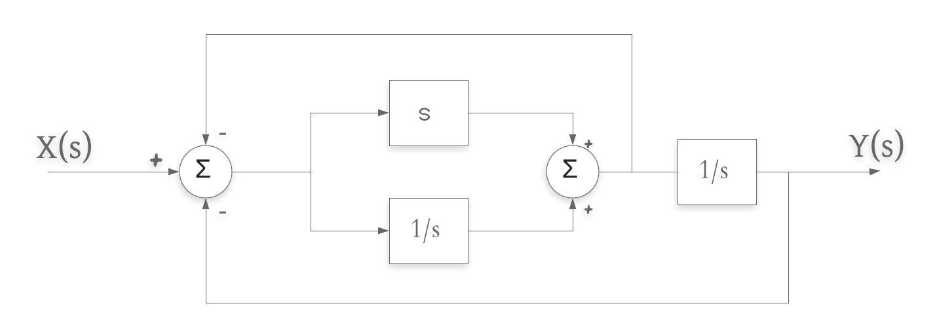
\includegraphics[width=0.8\textwidth]{pic1.png}
\end{figure}
(A) H(s)=$\frac{s^2+1}{s^3+s^2+s+1}$ \\
(B) H(s)=$\frac{s^2+1}{s^3+2s^2+s+1}$ \\
(C) H(s)=$\frac{s^2+1}{s^2+s+1}$ \\
(D) H(s)=$\frac{s^2+1}{2s^2+1}$
\end{frame}

\begin{frame}{Solution}
Here we have two transfer function s and $\frac{1}{s}$ in parallel with a adder as shown in figure.
After solving these two parallel transfer function by just adding both of them we will get
\begin{figure}
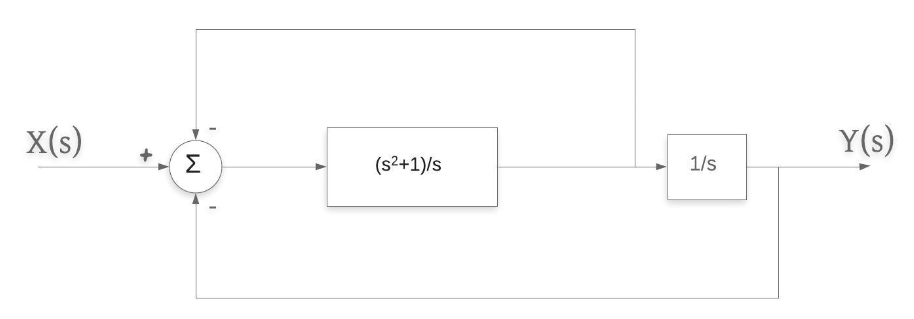
\includegraphics[width=0.8\textwidth]{pic2.png}
\end{figure}
\end{frame}

\begin{frame}{Solution}
Now we will convert three input adder into two input adder as shown in figure given below.
\begin{figure}
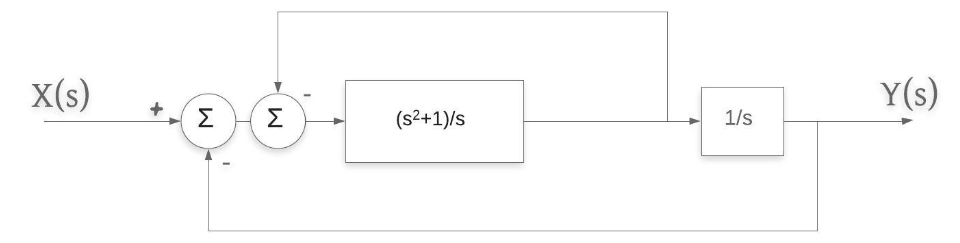
\includegraphics[width=0.8\textwidth]{pic3.png}
\end{figure}
\end{frame}

\begin{frame}{Solution}
Now we have Negative Unity Feedback System(NUFS) in closed loop transfer function. \\Let's say we have transfer function G(s) with Negative Unity Feedback System in closed loop then we will solve this by\\             \\ $\frac{G(s)}{1+G(s)}$.
\\Here we have
\begin{figure}
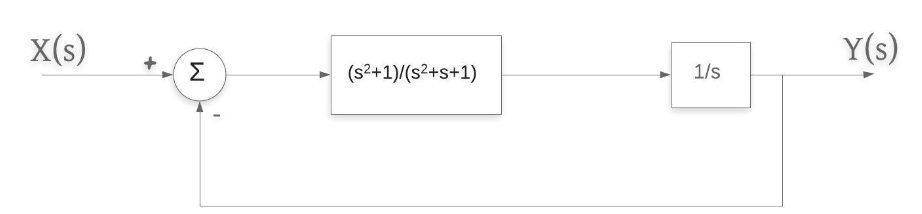
\includegraphics[width=0.8\textwidth]{pic4.png}
\end{figure}
\end{frame}

\begin{frame}{Solution}
Here we have two transfer function in series 
\begin{figure}
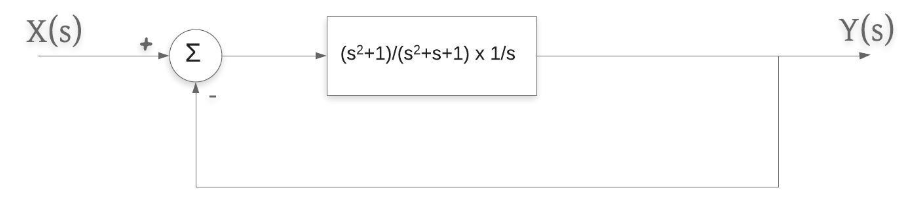
\includegraphics[width=0.8\textwidth]{pic5.png}
\end{figure}
\end{frame}

\begin{frame}{Solution}
Now we have one more transfer function with negative unity feedback.
\begin{figure}
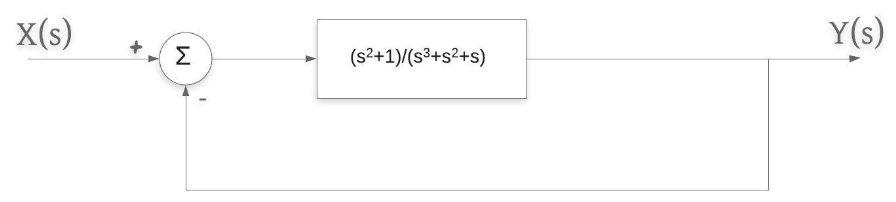
\includegraphics[width=0.8\textwidth]{pic6.png}
\end{figure}
Again we will solve this then we will get
\begin{figure}
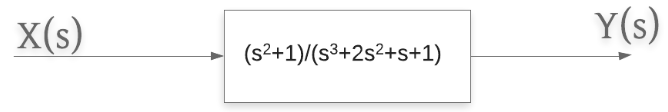
\includegraphics[width=0.8\textwidth]{pic8.png}
\end{figure}
\end{frame}
\begin{frame}{Solution}
Now\\

X(s)($\frac{s^2+1}{s^3+2s^2+s+1}$)=Y(s)\\

$\frac{Y(s)}{X(s)}$=$\frac{s^2+1}{s^3+2s^2+s+1}$\\
 The correct option is (B)
\end{frame}
\end{document}